\documentclass{standalone}
\usepackage{tikz}
\usepackage{amsmath}

\begin{document}
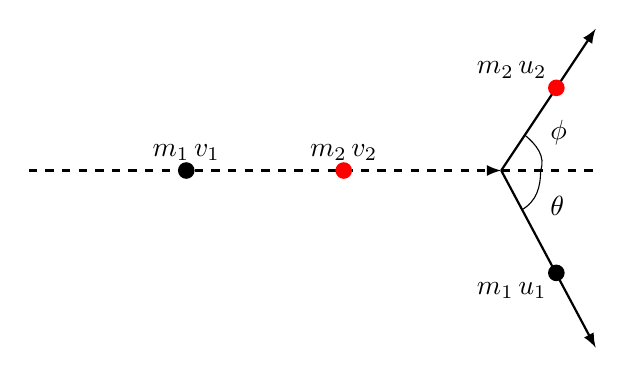
\begin{tikzpicture}

    
    \draw[thick,-latex,dashed] (0,2) -- (6,2);
    \draw[thick, dashed] (6,2) --(7.2,2);
    
    \draw[thick, -latex] (6,2) -- (7.2,3.8);
    \draw[thick, -latex] (6,2) -- (7.2,-0.25);

    \draw[] (6.5,2)  to[out=70, in=320](6.3,2.45);
    \node[above right] at(6.5,2.2){$\phi$};
    \draw[] (6.5,2)  to[out=270, in=30](6.26,1.5);
    \node[below right] at(6.5,1.8){$\theta$};
    
    \fill[black] (2,2) circle (3pt);
    \fill[red] (4,2) circle (3pt);
    \fill[red] (6.7,3.05) circle (3pt);
    \fill[black] (6.7,0.7) circle (3pt);

    \node[above] at(2,2){$m_1\,v_1$};
    \node[above] at(4,2) {$m_2\,v_2$};
    \node[above left] at(6.7,3.05) {$m_2\,u_2$}; 
    \node[below left] at(6.7,0.7){$m_1\,u_1$};
\end{tikzpicture}
\end{document}
